Essential components of the \CodeName ecosystem will be described and discussed in the following chapter, which includes the core configuration of the system, such as accessibility and mounting points. Other essential components counts; the delegation framework and the foundation package including the \texttt{SofaBaseObject} and the operation context definition.

\section{System configuration} \label{sec:configuration}
Each instance of \CodeName running is specified by a set of different parameters in the configuration file. All parameters are chosen, defined and implemented in order to make each version as customizable as possible. Figure \ref{fig:cfg_example} is an example of a custom implementation of a \CodeName configuration.
\newline

Each configuration specification is written in a \texttt{.cfg} file format (explained in definition \ref{def:cfg})) with four predefined groups:
\begin{itemize}
	\item \textbf{general}: Used to define various thresholds, retries, and path, but most important the \texttt{instance-name} which differentiates this instance from the rest. Additionally, it enables virtualization (described in section \ref{sec:virtualization}) and recovery (described in section \ref{sec:recovery}).
	\item \textbf{gateway/storage/monitor}: Used to specify the addresses and pots of the three different nodes booted at startup.
\end{itemize}

The language chosen could have been YAML \cite{PageYaml} or even JSON, but the readability and white space insensitivity of config files was preferred.

\begin{figure}
\vspace*{4mm}
\begin{lstlisting}[language=bash, frame=single, basicstyle=\ttfamily\tiny, otherkeywords={[,],=}, numbers=none, deletekeywords=enable]
[general]
project-path = /code/sofa-project/sofa
log-file = /code/sofa-project/sofa.log
keyspace-size = 2**5
mount-point = /mnt/sofa/
instance-name = exampledata

# Defined in seconds
heartbeat-scheduler-delay = 1
num-heartbeat-retries = 5
enable-live-software-reboot = True

load-balancing-threshold = 1

# Defined in megabytes
block-size = 5.0

[gateway]
addresses = localhost:9999

[storage]
addresses = localhost:8888

[monitor]
addresses = localhost:7777
\end{lstlisting}

\caption{Example of a \CodeName configuration implementation \label{fig:cfg_example}}
\end{figure}

\vspace*{4mm}
\begin{definition}[.cfg] \label{def:cfg}
\textit{A commonly used generic preference file for parameters and initial settings for an application, which is defined in a flat text file format, with minor syntactic features such as groups.}
\end{definition}
\vspace*{6mm}

It is important to notice that the \texttt{block-size} parameter defines that maximum allowed size for any given block of data and not a fixed size for each, as this would violate following objective described in section \ref{sec:objectives}:

\begin{quotation}
	\textit{"To store data in arbitrary sized chunks as a consequence of above mentioned."}
\end{quotation}

Other configuration parameters such as \texttt{heartbeat-scheduler-delay} and \texttt{enable\-live-software-reboot} will be described and deliberated on as part of the components they strengthen.

\section{\texttt{SofaBaseObject}} \label{sec:sofabaseobject}
Dataset in \CodeName has to adhere the interface defined in the \texttt{SofaBaseObject}, which is composed and designed in such a way that the associated data potentially\footnote{Vastly depended on how the function from the interface is implemented.} is stored and processed optimally.

\vspace*{5mm}
A dataset is defined by a number of properties:
\begin{itemize}
	\item A unique \textbf{name} that will be used to identify it, throughout the lifetime of the dataset in \CodeName.
	\item An optional \textbf{description} parameter to differentiate between and recognize dataset with similar or ambiguous names.
	\item Optional list of \textbf{operation context}s (described subsequently in section \ref{sec:operation} in this chapter) to be executed on the data.
\end{itemize}
\vspace*{5mm}

, and a number of required, and optional functions that will be discussed and described in details throughout the rest of this section since it is crucial to understand how, what seems like a limiting amount of functions, is general and generic enough to describe any type of data and operations to be executed on it. The meaning of the term \textit{operation (context)} and the purpose will be described subsequently in this chapter in section \ref{sec:operation}. 
\newline

Figure \ref{fig:preprocess-nextentry} illustrates the context of which following required and optional functions: \textbf{preprocessing}, \textbf{next entry}, \textbf{replication factor} and \textbf{distribution strategy} are used in the flow of adding new data (the append API\footnote{Application Programming Interface} will be described in chapter \ref{chp:api}).

\begin{figure}
	\centering
	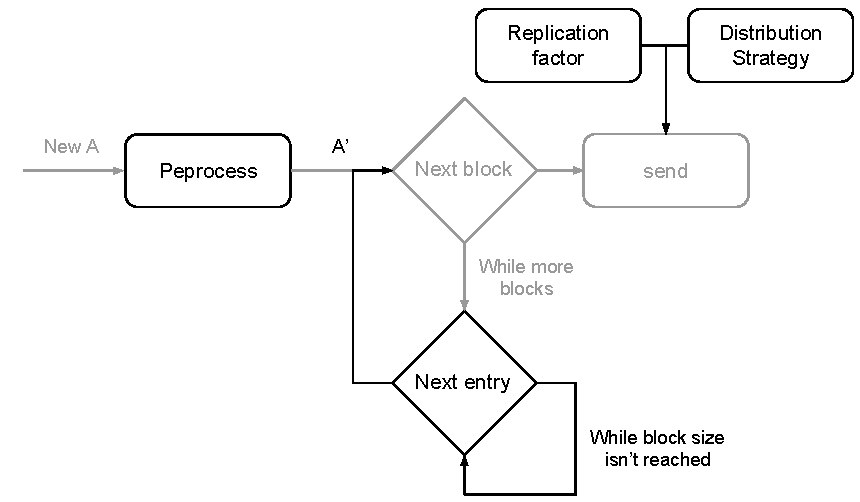
\includegraphics[scale=0.8]{pdf/preprocess-nextentry.pdf}
	\caption[\texttt{SofaBaseObject} interface functions]{Illustration of where some of the \texttt{SofaBaseObject} interface functions are used. The ones depicted in a light shade of gray are other key parts of the append operation that will be described later in chapter \ref{chp:api}: Core API. \label{fig:preprocess-nextentry}}
\end{figure}	

\subsection{Prepossessing}
A step that is executed initially when new data is added to \CodeName before it is split. This step facilitates options\footnote{Built-in \CodeName function to load data from local path or url are provided and accessible through the \texttt{SofaBaseObject} API.} such as reshaping data array if they are fetched over network or loading the data as a specific object type.

\subsection{Next entry}
The purpose of this function is to transition the responsibility of split the data correctly towards the end-user, rather than imperfection choices by the system. With this approach, \CodeName relies on the users know-how and expertise regarding the internal structure of the data and how to split it semantically correct, such that coherent parts are jointly stored.
\newline

The consideration and complexity behind this required function and its role as part of the append-flow (depicted in figure \ref{fig:preprocess-nextentry}) jointly contribute to a generic solution that optimally will accomplish following objective described in section \ref{sec:objectives}: 

\begin{quotation}
	\textit{"Split data such that semantically coherent parts are stored jointly and thus eliminating the data residual problem known from Hadoop."}
\end{quotation}
\vspace*{3mm}

While the users now have been granted some, not unreasonable responsibilities are \CodeName on the other hand in control of combining semantic blocks and distributing them concerning the distribution strategy and replication factor.

\subsection{Distribution strategy}
\CodeName provides three different distribution strategies for the semantic blocks, the strategies are offered at a data level and not at a system wide level as in many other alternatives, such that it can be tailored ideally to each specific use-case. The three ones are:

\begin{enumerate}
	\item \textbf{1-by-1}: A basic implementation of the Round Robin distribution and scheduling algorithm (outlined in definition \ref{def:rr}).
	\item \textbf{Tiles}: Extended version of the Round Robin algorithm with support for \textit{n}-by-1, such that semantic blocks are tiled/grouped by \textit{n} before distribution.
	\item \textbf{Linear}: A specific single run-through version of the tiles strategy algorithm described above, where the blocks are distributed as equally as possible\footnote{ Eq: $\lceil blocks / storage\_nodes\rceil$, to make sure that there isn't an overabundant of blocks on last server (\CodeNameShort's interpretation of \textit{'last'} server will be explained subsequently in chapter \ref{chp:api}).} across the storage nodes.
\end{enumerate}
\vspace*{5mm}

\begin{figure}[ht!]
	\centering
	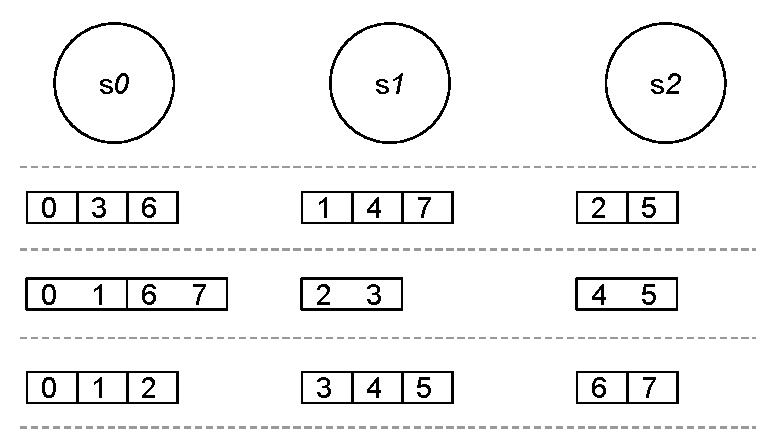
\includegraphics[scale=0.85]{pdf/distribution-strategies.pdf}
	\vspace*{3mm}
	\caption[Distribution strategies]{An example of how the three distribution strategies work in action. The figure illustrates three storage nodes denoted by s\textit{0}, s\textit{1} and s\textit{2} and the block stored on them with strategies of respectively \textbf{1-by-1}, \textbf{Tiles} of size 2 and \textbf{Linear}. \label{fig:distribution-strategies}}
\end{figure}	

It is worth to notice that all the different distribution strategies in one or another way are a variant of the Round Robin algorithm and thereby adhere to the architecture and design criterion for partitioning and distribution described in section \ref{sec:pandd}.
\newline

Although the strategies initially appear to be approximately equal, the results of appending eight blocks on three storage nodes are very divergent (result depicted in figure \ref{fig:distribution-strategies}) and thus one could easily find very different purposes for each:

\begin{quotation}
Data with an extensive interrelationship between blocks are a straightforward example of where a tiled strategy would be preferable, since operations on such data usually would require a considerable amount of exchanges of ghost points with the neighbors (a technique Wilkinson \etal covers in \cite{Wilkinson:1998:PPT:289352} and that will be explained in section \ref{sec:operation}) to produce the expected results. Even though a linear distribution strategy also would work for this purpose, it is a requirement that the total number of blocks are known on beforehand, since data is streamed into \CodeName.
\end{quotation}

One could think of other distribution strategies and algorithms to use on certain specific types of data, hence its an ambition subsequently to design and come up with a generic interface for defining individual strategies and algorithms.

\subsection{Replication}
\CodeName provides the opportunity of virtual replication at a data level specified independently for each dataset. Compared to other alternatives as the ones evaluated in section \ref{sec:related} such as Hadoop this is a unique and contemporary privilege, since replication commonly is at a machine level. Preceding enables options for prioritizing datasets with regards to importance and reproducibility of data.
\newline

The replication factor can additionally be used as a load balancing mechanism for the dataset and thereby increase its accessibility for the end-users, this among other things were described and discussed in section \ref{sec:delegation}.

\section{Operation context} \label{sec:operation}
An \texttt{OperationContext} is a mutable object attached to a dataset that represents and describes a function or multiple chained ones and the associated parameters and prerequisites, to be executed on the data. A number of optional specifications are available such that most most common requirements are supported out of the box to increase productivity and correctness.
\newline

The syntax for characterizing this object, the optional specifications, and a lot more will be examined in details throughout the rest of this section since it is crucial to understand too, like the other foundation object \texttt{SofaBaseObject} described in section \ref{sec:sofabaseobject}.

\subsection{Sequential / Parallel}
Functions of an operational context can be grouped in an unlimited amount of nested sequential and parallel containers, although it is required that the outer most container is of the sequential type. The two code snippets in the forthcoming \textbf{syntax} sections exemplifies the usage of these two varies.

\subsection{Syntax}
The \texttt{OperationContext} object can be instantiated in two ways depending on the end-users preferences:
\vspace*{2mm}

\begin{enumerate}
	\item In a traditional fashion way:
\vspace*{2mm}
\begin{lstlisting}[language=Python, basicstyle=\footnotesize, numbers=none, showtabs=false, showstringspaces=false, showspaces=false, 
otherkeywords={[,{,},],Sequential,Parallel,OperationContext}, deletendkeywords={sum}]
OperationContext(Sequential(Parallel(
                            Sequential(count, sum), 
                            Sequential(count_nocase, sum)
                           ), equality))
\end{lstlisting}
\vspace*{-2mm}
	\item And the effective customizable shorthand version:
\vspace*{2mm}
\begin{lstlisting}[language=Python, basicstyle=\footnotesize, numbers=none, showtabs=false, showstringspaces=false, showspaces=false, 
otherkeywords={[,{,},],Sequential,Parallel,OperationContext}, deletendkeywords={sum}]
OperationContext.by('[{[count, sum], 
                       [count_nocase, sum]
                      }, equality]')
\end{lstlisting}
\vspace*{-2mm}
	The sequential (\texttt{[} and \texttt{]}) and parallel operators (\texttt{\{} and \texttt{\}}) are the default ones but are changeable as long as they all four are distinct and aren't string definition syntax operators, such as \texttt{'} and \texttt{"} as in most common programming languages.
\end{enumerate}

\subsection{Ghosts}
In \cite{Wilkinson:1998:PPT:289352} Wilkinson \etal covers the technique of ghost points which is a procedure well studied and used in high performance computing, etc. Common computing challenges where this is superior are typically situations where the data has an immense correlation between the semantic blocks such as image data or climate simulation results, as previously described. 
\newline

Figure \ref{fig:ghost-points} illustrates the fundamental idea behind ghost points also denoted as halo lines where each domain has an extra row of data added at the boundary between the others consisting of data from the neighbor. 

\begin{figure}[ht!]
	\centering
	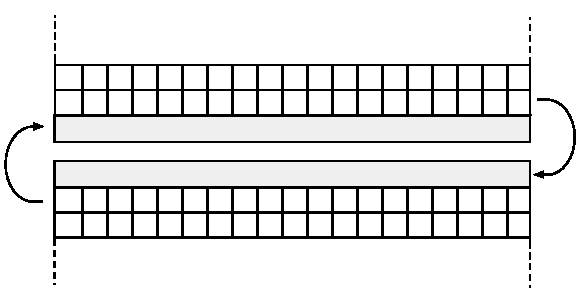
\includegraphics[scale=0.92]{pdf/ghost-points.pdf}
	\vspace*{3mm}
	\caption{Fundamental idea of ghost points \label{fig:ghost-points}}
	\vspace{2mm}
\end{figure}	

One or more rows are exchanged between neighbors in order to compute the accurate results beyond everything, but also to minimize the I/O-cost compared to exchanging data independently when needed.
\newline

\begin{figure}[ht!]
\centering
\vspace*{6mm}
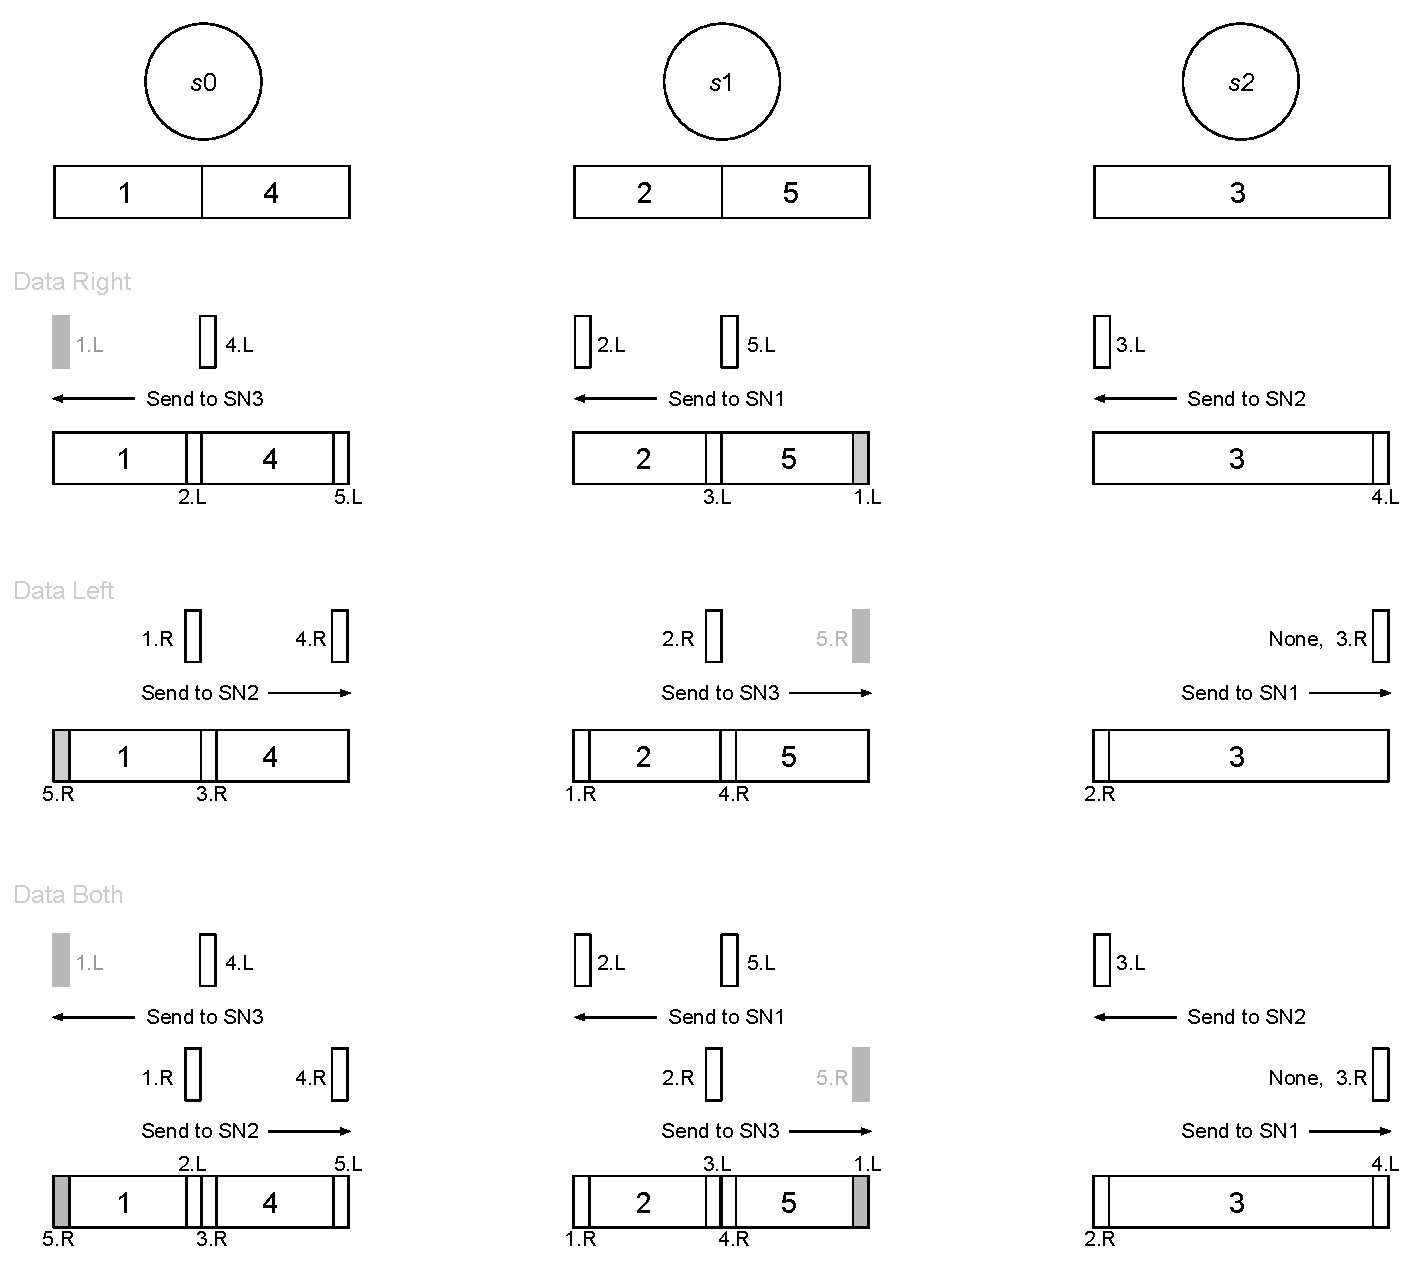
\includegraphics[scale=0.55]{pdf/ghost-transfer.pdf}
\vspace*{4mm}
\caption[Ghost transfer example]{Example of how ghost points are transferred between nodes.}
\vspace*{6mm}
\label{fig:ghost-transfer}
\end{figure}

Figure \ref{fig:ghost-transfer} illustrates the flow of the three supported types of ghost point exchange in \CodeName:

\begin{enumerate}
	\item Sending data clockwise / \textbf{right}.
	\item Sending data counterclockwise / \textbf{left}.
	\item And in \textbf{both} directions with symmetric and asymmetric semantic units as ghosts.
\end{enumerate}
\vspace*{2mm}
, though, there is a limitation held in common by all three of them; that data \textbf{overflow} from first to last when transferring left and last to first when transferring right aren't implemented for the time being.
\newline

The neighbor exchange protocol is implement by default in \CodeName and can be utilized in two different ways:

\begin{enumerate}
	\item As a \textbf{preprocessing} step for operations where ghosts are demanded initially.
	\item Moreover, as a built-in keyword function\footnote{Defined and explained later in this section.} used as an intermediate step before a function requiring ghosts in the chain of functions.
\end{enumerate}

\subsubsection*{Protocol}
The naïve approach for implementing a ghost point distribution protocol using Figure \ref{fig:sofa-overview} as starting point is to:
\begin{enumerate}
	\item First of all, let the gateway initialize the process at the root node\footnote{The definition of a root node for a dataset is defined in section \ref{sec:gateway} in an forthcoming chapter} for that particular dataset.
	\item Moreover, let that node initialize the calculation and exchange protocol on all the nodes with segments of the data.
	\item Finally, every storage node ask every neighbor for their needs in terms of ghost semantic blocks.
\end{enumerate}
\vspace*{2mm}
Such procedure as explained above requires a minimum of $5n-1$ I/O requests which is rather suboptimal. In distributed systems the focus is on optimizing the number of those requests and one could easily think of an optimized solution such as the one illustrated at Figure \ref{fig:ghost-v1}. 

This solution, which improves number of initialization requests (from $n-1$ to $n/2-1$) among others, requires $\frac{5}{2}n-1$ I/O operations which is a remarkable improvement compared to the previous amount.

\begin{figure}[ht!]
	\centering
	\vspace*{3mm}
	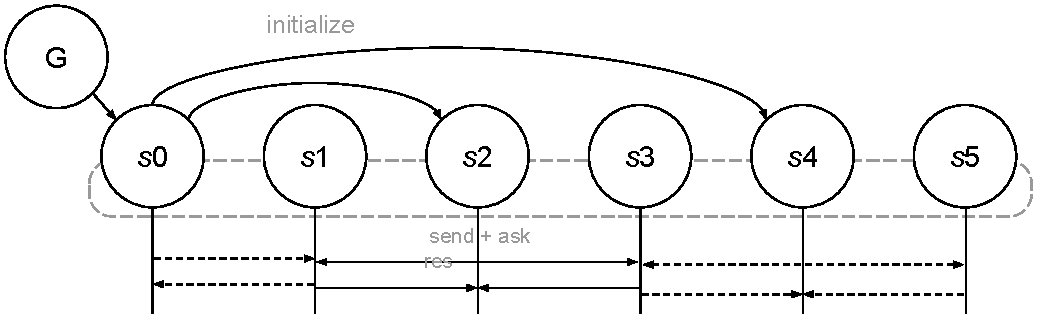
\includegraphics[scale=0.68]{pdf/ghost-v1.pdf}
	\caption{Ghost protocol v2: Initial design and thoughts \label{fig:ghost-v1}}
	\vspace*{3mm}
\end{figure}	

However, in high performance computing (HPC) clusters as this prototype framework first and foremost is targeted (as mentioned in section \ref{sec:hardware}) it is a matter of time steps and not I/O as such for which the HPC solution illustrated at Figure \ref{fig:ghost-final} is most optimal.
\newline

\begin{figure}
	\centering
	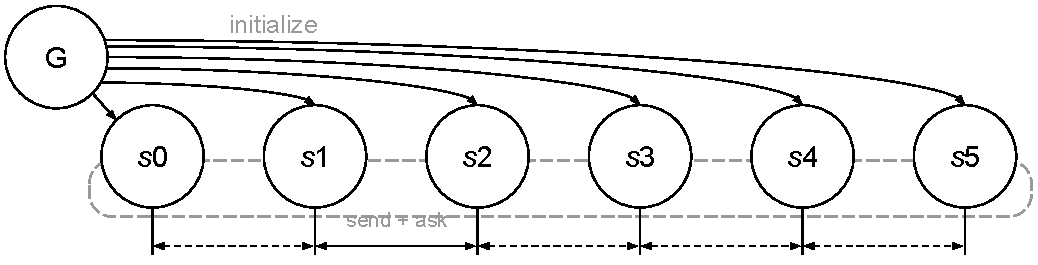
\includegraphics[scale=0.68]{pdf/ghost-final.pdf}
	\caption{Ghost protocol v3: The HPC solution \label{fig:ghost-final}}
\end{figure}	

This solution implements a \textit{"send fast, receive late"}-terminology based broadcast storms\footnote{Requires reasonable network and communication library implementation to be an improvement to prior solutions.} on the prior knowledge that every node knows what the two neighbors needs (regarding ghost semantic blocks), due to the scalable access model where all storage components at real-time can calculate others ids and thereby requirements. The broadcast storm is superior in highly synchronous environments like this where everybody can calculate and send at the same time and equivalently for receiving and thus utilizing the network bandwidth the most. 

\subsection{Postprocessing}
An optional step executed after the core of the operation has completed and before the end-user gets the result. This step facilitates options such as filtering or plotting data to produce quality figures on-the-fly at once.

\subsection{Built-in keywords}
\CodeName offers a range\footnote{Effortlessly extended when demanded} of different built-in keyword functions for conventional operations on data along with a module importer library that easily binds language specific core functions to \CodeName operations and functions, with a function name change if requested.

An example: \texttt{count(}x, y\texttt{)} is a built-in function from the \texttt{string} module in Python \cite{PagePython} that counts number of \texttt{y} in \texttt{x}. Following snippet transforms the \texttt{count(}x, y\texttt{)} into \texttt{count\_occurrences(}x, y\texttt{)} with identical logic parameters and results:
\vspace*{2mm}
\begin{lstlisting}[language=Python, basicstyle=\footnotesize, numbers=none, showtabs=false, showstringspaces=false, showspaces=false, otherkeywords={string,new_fun_names}, stringstyle=\color{blue}]
   module_binder(string, function_binder, ['count'], 
                 new_fun_names=['count_occurrences'])
\end{lstlisting}

Noticeable keyword to discussed and elaborate on are:
\vspace*{2mm}

\begin{itemize}
	\item The \textbf{modify} keyword function takes one argument defined by a semicolon: \texttt{modify:<function\_name>} and calls the action defined by the \texttt{function\_name} parameter with the current data block state. The modify function is especially useful in combination with the module importer service since it is quite often that general core functions require that data to be in a certain format.
	\item \textbf{neighborhood} takes either zero, one or two arguments\footnote{Separated by a semicolon as for the other keyword functions.} and implements the ghost point transfer protocol described previously in this section.
	\begin{enumerate}
		\setcounter{enumi}{-1}
		\item \texttt{neighborhood}
		\item \texttt{neighborhood:ghost\_count}
		\item \texttt{neighborhood:left\_ghost\_count:right\_ghost\_count}
	\end{enumerate}
	The default value of \texttt{neighborhood} is \texttt{neighborhood:1}, which again is a equivalent to \texttt{neighborhood:1:1}. The function with two arguments mainly cohere asymmetric counts, \ie \texttt{left\_ghost\_count} $\neq$ \texttt{right\_ghost\_count}.	
\end{itemize}

\section{Delegation} \label{sec:delegation}
The delegation framework in \CodeName serves a vast amount of important practical and approachable purposes:
\begin{itemize}
	\item The responsible dispatcher part (illustrated at Figure \ref{fig:delegation-framework}) is pledged to route the request to the node responsible for it.
	\item Count the number of delegation-important\footnote{\label{note:explained}Will be explained and thereby be more obvious subsequently in this section.} operations that are executing simultaneously.
	\item To forward the request to the next replica\footnote{\label{note:replication-factor}If \texttt{replication factor} is larger than one.} in the \textbf{forward queue} if the local operation count is larger than the specified threshold\footnoteref{note:explained}.
	\item Moreover, to redirect the request to the next replica\footnoteref{note:replication-factor} in the \textbf{redirect queue} if the request requires replication.
\end{itemize}
\vspace*{4mm}

\begin{figure}[ht!]
	\centering
	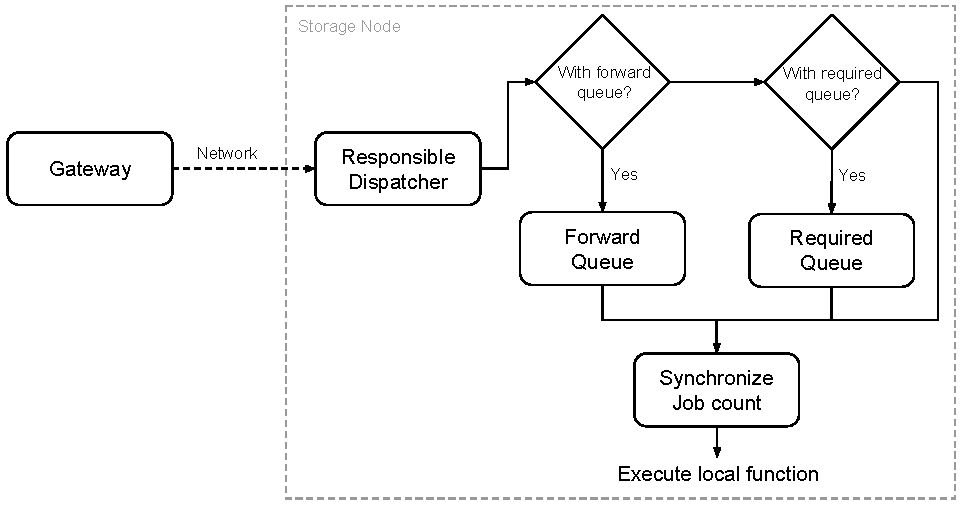
\includegraphics[scale=0.72]{pdf/delegation-framework.pdf}
	\caption[Overview of the delegation framework]{Overview of the flow in the delegation framework. \label{fig:delegation-framework}}
\end{figure}	

\noindent
The framework is invented to:
\begin{itemize}
	\item Simplify the usage of individual dataset replication and seal the logic described as part of section \ref{sec:sofabaseobject}.
	\item Streamline the offloading of the primary data replicas when needed\footnoteref{note:replication-factor}.
	\item Enables a dynamic load balancing (whilst the DM Multipath described in \ref{sec:recovery} provides load balancing on a disk level) on separate datasets by the \texttt{load\-balancing-threshold} in the configuration file (described in section \ref{sec:configuration}) in combination with the replication factor.
\end{itemize}
\vspace*{4mm}
The delegation solution is designed as illustrated in Figure \ref{fig:delegation-framework} and is integrated into the core of storage nodes logic (defined in section \ref{sec:storage}). The responsible dispatcher is theoretically optional to use but is enforced by default, provided that it is debilitated it would require the gateway (described in section \ref{sec:gateway}) to be aware of how to determine the responsible server\footnote{Equation \ref{eq:responsible}} for the particular dataset, which would violate the single point of failure (SPOF) objective listed in section \ref{sec:objectives}:
\begin{quotation}
\textit{"Eliminating single-point of failure on a stateful master server."}
\end{quotation}
, since the gateway then would require slightly more discernment than expected for a stateless server\footnote{\label{note:stateful}A stateful server is commonly a synonym with SPOF.}.
\newline

The responsible server is calculated based on following calculation (\ref{eq:responsible}), and the current server is executing the function if the result is equal to this. Otherwise, the request is routed to the responsible.
\begin{equation} \label{eq:responsible}
\Big(\Big\lfloor\dfrac{\texttt{id}:data}{\texttt{\#}keyspace}\Big\rfloor + \texttt{id}:replica\Big) \texttt{ mod } \texttt{\#}storagenodes
\end{equation}

\subsubsection*{Protocol}
A range of different opportunities are examined, reviewed, and some tested to implement such framework as described. The first choice was to design a gossip based protocol as Tanenbaum \etal examines in \cite{Tanenbaum:2006:DSP:1202502} between gateways to let the others know what "\textit{you}" are doing. Such a protocol will in \textbf{best case} improve performance since the gateways will be capable of predicting which server to send the request to, \textbf{worst case} on the other hand would not be different from the default behavior and thus not affecting the correctness of the results.
\newline

Preceding protocol was first of all discarded due to the increased complexity in logic on the gateway servers and the sudden intercommunication between them that it would cause, and secondly because it would require the servers to be moderately stateful\footnoteref{note:stateful}.

\begin{quotation}
C. A. R. Hoare defined in his 1978 paper \textit{"Communicating Sequential Processes"}\cite{Hoare:1978:CSP:359576.359585} a formal language for describing patterns of interaction in concurrent systems, which later has been implemented in a variety of different well known programming languages such as Python by Bj{\o}rndalen, Vinter \etal in \cite{bjorndalen2007pycsp}.
\end{quotation}

\noindent
Although this second approach currently is not achievable since it would require that \CodeName is implemented in a CSP fashion with processes and channels, it is from a theoretical perspective an interesting thought and therefor included as a conceptual task. One could think of a \CodeName system based on CSP techniques with channels between gateways and storage nodes and the forward queue to load balance the system, for example, implemented as an Alternative (explained in definition \ref{def:alternation}) that facilitates a solution without queues and with improved I/O.
\vspace*{3mm}
\begin{definition}[PyCSP: Alternative] \label{def:alternation}
\textit{A central abstraction as Bj{\o}rndalen, Vinter \etal describes in \cite{bjorndalen2007pycsp} that from a list of channels selects the one ready (for a read or write) the first and thus implements a first-come-first-serve strategy.}
\end{definition}

The model implemented is a comprise between complexity, time and expected outcome compared to the fact that this initial \CodeName implementation was purposed as a prototype to a plausible solution. It is an extended dynamic store and forward method where whole requests are redirected to a random storage node as explained in details in section \ref{sec:gateway}, which if needed based on responsible dispatcher either is executing or forwarding the request. 
\newline

Assuming forwarding is enabled based on the conditions previously listed and the primary replica has enough work to do, it will generate the forward queue based on a number of parameters and forward the request to the first in the queue. A worst case example is as follows:
\vspace*{-5mm}
\begin{center}
\begin{align*}
	0: &x \rightarrow [1, 2, 0] \\
	1: &x \rightarrow [1, 0] \\
	2: &x \rightarrow [0] \\
	0: &x \rightarrow []
\end{align*}
\end{center}
, where three storage nodes ($0 \ldots 2$), $0$ as the dataset root and a generated forward queue as $[1, 2, 0]$ is assumed. The reason why the node it self is added at the end of the queue, is precisely the case listed above were all the other nodes is occupied too and the root node receives an empty list, and is forced to execute the operation itself.
